%!TEX root = forallxyyc.tex

% Bastard Title

\pagestyle{empty}

%\vspace*{80pt}

\begin{raggedleft}
     \vspace*{1cm}
      \hfill
     \sffamily\fontsize{40pt}{0pt}\selectfont %V2
     % \color{lyallpink}
      %\textbf{Para Tod{\fontsize{56pt}{0pt}\selectfont\rmfamily\hspace{-2pt}\textit{x}}\hspace{-3.5pt}s} %V1
      \textbf{Para Tod{\fontsize{49pt}{0pt}\selectfont\rmfamily\hspace{-3.5pt}\textit{x}}\hspace{-1.5pt}s}                   
      \vskip.5cm
          
      \sffamily\fontsize{28pt}{0pt}\selectfont %V1
      \uppercase{\textbf{Natal}} %V2
      
      %\definecolor{beaublue}{rgb}{0.33, 0.33, 0.33}
      \color{black}
      \vspace*{1cm}
      \sffamily
      \fontsize{21pt}{20pt}\selectfont
      \textbf{uma introdução à\\ lógica formal}

 
 \vfill
\fontsize{12pt}{16pt}\selectfont \textit{De } \textbf{P.~D. Magnus}\\
\textbf{Tim Button}\\
\textit{com acréscimos de}\\
\textbf{J.~Robert Loftis}\\
\textbf{Robert Trueman}\\
\textit{remixado e revisado por}\\
\textbf{Aaron Thomas-Bolduc}\\ \textbf{Richard Zach}\\
\textit{adaptado, re-remixado, re-revisado e ampliado  pelo}\\ \textbf{Grupo de Estudos em Lógica da UFRN \\ (GEL--\textit{Carolina Blasio})}\\
%\href{https://gelogica.weebly.com/para-todxs-natal.html}{{\small link para a lista de coautores desta versão}}

\vfill

%\textbf{1ª Edição \ -- \ 21 de julho de 2022} \ \ \ \ \ \ \par
\textbf{1ª Edição }\\
{21/07/2022}\par
%\textbf{\today}\par
\end{raggedleft}

\begin{figure}[b]
  \begin{minipage}{0.33\textwidth}
%     \centering
%     \includegraphics[width=3cm, left]{./assets/logo-ufrn-escala-de-cinza}
     
\includegraphics[width=2.5cm, left]{./assets/logo-ufrn-flat}
  \end{minipage}%\hfill
  \begin{minipage}{0.33\textwidth}
     \centering
     
\includegraphics[width=2.5cm]{./assets/ppgfil-logo}
  \end{minipage}
  \begin{minipage}{0.33\textwidth}
     \centering
     
\includegraphics[width=2cm]{./assets/by}
  \end{minipage}%\hfill
\end{figure}

\newpage


\begin{figure}
\vspace*{8cm}
\centering
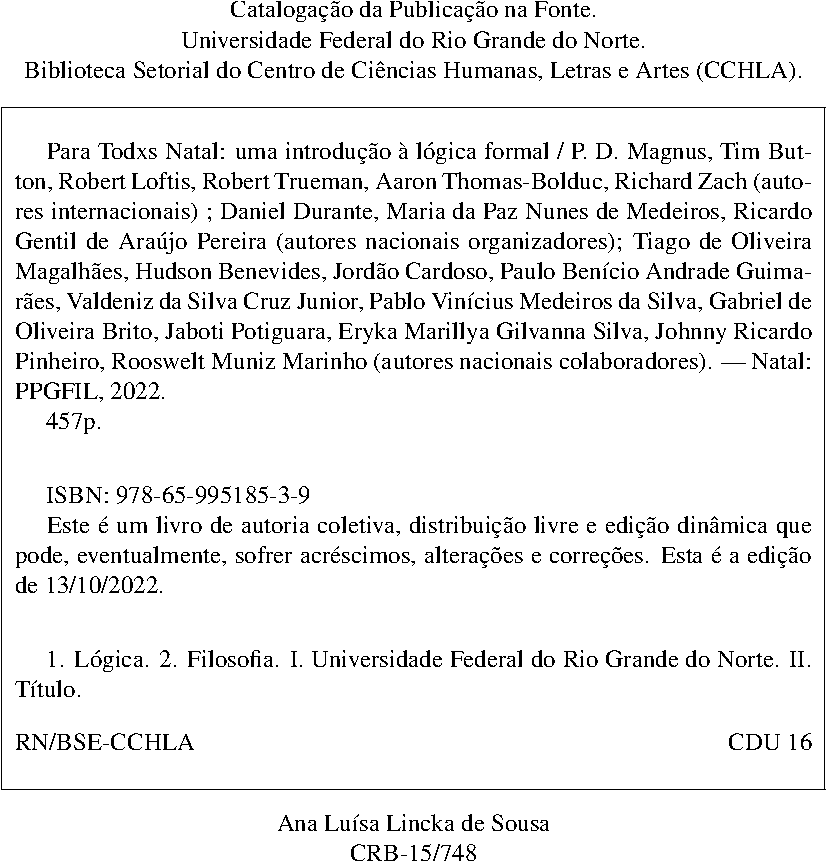
\includegraphics[width=8cm]{./assets/ficha-cat}
\end{figure}


\newpage

\thispagestyle{empty}
\onecolumn
\ 
\vfill

\parbox{3 in}{

Este é um livro de autoria coletiva, distribuição livre e edição dinâmica que pode, eventualmente, sofrer acréscimos, alterações e correções.
Esta versão é a correção de  \textbf{\mydate}\  da 1ª Edição (21/07/2022).
Você pode verificar neste link
\href{https://github.com/Grupo-de-Estudos-em-Logica-da-UFRN/Para-Todxs-Natal/blob/main/paratodxsnatal.pdf}{$\langle$última versão$\rangle$}
se alguma versão mais recente já está disponível.
Você pode também colaborar com o aprimoramento deste livro e tornar-se coautor ou coautora das próximas edições.
Caso encontre erros ou tenha sugestões de reescrita ou críticas, você pode enviá-los através deste formulário 
\href{https://forms.gle/yd4yH9WAo6TxAiSj8}{$\langle$correções e sugestões$\rangle$}.
Se alguma de suas sugestões for incorporada, ainda que seja apenas uma vírgula, seu nome será incluído na lista de coautores colaboradores das próximas edições. 

%Esta é a versão rascunho (0.8 -- \mydate) de um livro que ainda não está pronto.
%Você pode verificar neste link
%\href{https://github.com/Grupo-de-Estudos-em-Logica-da-UFRN/Para-Todxs-Natal/blob/main/paratodxsnatal.pdf}{$\langle$última versão$\rangle$}
%\hbox{\url{https://rb.gy/w3ovdf}}
%se alguma versão mais recente já está disponível.
%Este livro está sendo testado em algumas turmas de uma disciplina introdutória de lógica da UFRN e planejamos finalizar uma primeira edição para publicação ainda em 2021. 
%A versão atual já contempla todo o conteúdo pretendido, mas o livro, de autoria coletiva, está em processo de revisão e ainda sofre com certa falta de padronização de notação e nomenclatura, falta de homogeneização do tom, além de muitos erros de escrita e digitação.
%Você pode nos ajudar na revisão e fazer parte do coletivo de coautores e coautoras reportando erros, críticas e sugestões neste formulário
%\href{https://forms.gle/yd4yH9WAo6TxAiSj8}{$\langle$correções e sugestões$\rangle$}
%\hbox{\url{https://forms.gle/yd4yH9WAo6TxAiSj8}} 
}

\newpage

\section{Lista de coautores da correção de \ \mydate}

{\small \subsection{Autores Internacionais}
\begin{itemize}
	\item P. D. Magnus \ \  (autor do \forallx)
	\item Tim Button \ \ (autor do \forallx: \textit{Cambridge})
	\item Robert Loftis \ \ (coautor do \forallx: \textit{Calgary})
	\item Robert Trueman \ \ (coautor do \forallx: \textit{Calgary})
	\item Aaron Thomas-Bolduc \ \ (coautor do \forallx: \textit{Calgary})
	\item Richard Zach \ \ (coautor do \forallx: \textit{Calgary})
\end{itemize}
  
\subsection{Autores Nacionais (organizadores)}
\begin{itemize}
	\item Daniel Durante 
	\item Maria da Paz Nunes de Medeiros
	\item Ricardo Gentil de Araújo Pereira
\end{itemize}

\subsection{Autores Nacionais (colaboradores)}
\begin{itemize}
	\item Tiago de Oliveira Magalhães
	\item Hudson Benevides
	\item Jordão Cardoso
	\item Paulo Benício Andrade Guimarães
	\item Valdeniz da Silva Cruz Junior
	\item Pablo Vinícius Medeiros da Silva
	\item Gabriel de Oliveira Brito
	\item Jaboti Potiguara
	\item Eryka Marillya Gilvanna Silva
	\item Johnny Ricardo Pinheiro
	\item Roosewelt Muniz Marinho
\end{itemize}}

\newpage

\noindent Esta obra é baseada no livro \href{https://github.com/rzach/forallx-yyc}{Forallx: \textit{Calgary}} de P.D. Magnus, Tim Button, J. Robert Loftis, Robert Trueman, Aaron Thomas-Bolduc e Richard Zach, que foi utilizado aqui sob a licença \href{https://creativecommons.org/licenses/by/4.0/}{CC BY 4.0}.
Mas para você entender direito a autoria deste livro, é preciso listar alguns outros livros e explicar a relação entre todos eles.

\begin{enumerate}
   \item \forallx, de P.D. Magnus

   \item \forallx: \textit{Cambridge}, de Tim Button

   \item \forallx: \textit{Calgary} de P.D. Magnus, Tim Button, J. Robert Loftis, Robert Trueman, Aaron Thomas-Bolduc e Richard Zach
   
   \item \textit{Metatheory}, de Tim Button
   
   \item  \forallx: \textit{Lorain Conty Remix}, de Cathal Woods e J. Robert Loftis
   
   \item \textit{A Modal Logic Primer}, de Robert Trueman
\end{enumerate}

\noindent A história é a seguinte.
P. D. Magnus escreveu o livro (1). Tim Button produziu o livro (2) baseado no livro (1) e Aaron Thomas-Bolduc junto com Richard Zach produziram  livro (3) com base no livro (2).
Mas Thomas-Bolduc e Zach também utilizaram materiais dos livros (1), (4), (5) e (6) na produção do livro (3).
%Aí nós, do \href{https://gelogica.weebly.com/}{GEL\,--\,\textit{Carolina Blasio}} (Grupo de Estudos em Lógica do Departamento de Filosofia da Universidade Federal do Rio Grande do Norte), 
%utilizamos o livro (3) como texto base %---(2021-10-01)
%para a produção deste livro, que não é uma tradução, mas um livro baseado no livro (3), em que fizemos muitas modificações, inclusões e adaptações, tendo como foco e público-alvo estudantes de graduação em filosofia que, em geral, não gostam e não têm muita familiaridade com matemática.
Aí nós, do \href{https://gelogica.weebly.com/}{GEL\,--\,\textit{Carolina Blasio}} (Grupo de Estudos em Lógica do Departamento de Filosofia da Universidade Federal do Rio Grande do Norte), utilizamos o livro (3) como texto base para a produção deste livro, que é um híbrido entre uma tradução livre e uma adaptação. O núcleo do \forallx:\,\textit{Calgary} foi integralmente incorporado ao \textit{Para Todxs:\,Natal}: seu conteúdo e estrutura, o estilo da abordagem e o tom da escrita. Nosso trabalho em cada capítulo iniciava-se sempre como tradução que, mesmo sem preocupação com a literalidade, atinha-se ao conteúdo do texto original. Em muitos capítulos isso foi tudo que fizemos. Em outros tantos, porém, fizemos acréscimos, modificações e adaptações, todas motivadas pelas características de nosso público-alvo: estudantes de graduação de filosofia que, em geral, não gostam nem têm muita familiaridade com matemática.
Nossa experiência ao longo dos anos nos sugere que estudantes de filosofia se interessam mais e aproveitam melhor a lógica quando a estudam junto com filosofia da lógica. Procuramos, no \textit{Para Todxs:\,Natal}, amplificar os elementos de filosofia da lógica já presentes no livro (3) e adaptá-los às nossas concepções.
%---versões anteriores a (2021-10-01)
%para a produção deste livro, que não é uma tradução, mas uma adaptação livre, em que fizemos modificações, alterações e inclusões.
%Nossa adaptação foi feita tendo estudantes de graduação em filosofia como público-alvo.
%Nossa experiência ao longo dos anos nos sugere que  os estudantes de filosofia se interessam mais e aproveitam mais a lógica quando a estudam juntamente com a filosofia da lógica.
%O que fizemos, então, foi amplificar os elementos de filosofia da lógica que já est avam presentes no livro (3), e adaptá-los às nossas concepções.

\clearpage

\begin{figure}[t]

\includegraphics[width=2cm,center]{./assets/by}
\end{figure}

Os livros (1), (2), (3) e (4) estão todos sob a licença \href{https://creativecommons.org/licenses/by/4.0/}{CC BY 4.0}, e os livros (5) e (6) foram utilizados por Thomas-Bolduc e Zach com permissão.\label{cc4by}



%\bigskip

Esta obra está protegida sob a licença \href{https://creativecommons.org/licenses/by/4.0/}{Creative Commons \hbox{Attribution 4.0}}. 
Você é livre para copiar e redistribuir este material em qualquer meio ou formato, remixar, transformar e desenvolvê-lo para qualquer finalidade, mesmo comercialmente, nos seguintes termos:
\begin{itemize}\label{cc4by}
\item Você deve dar o crédito apropriado, fornecer um link para a licença e indicar se foram feitas alterações. Você pode fazê-lo de qualquer maneira razoável, mas não de maneira que sugira que os licenciantes (os demais autores) endossam você ou seu uso.
\item Você não pode aplicar termos legais ou medidas tecnológicas que restrinjam legalmente outras pessoas a fazer o que a licença permite.
\end{itemize}

\noindent A editoração gráfica deste livro foi produzida com base no código fonte \LaTeX{} do livro (3),  que está disponível em \hbox{\href{https://forallx.openlogicproject.org}{forallx.openlogicproject.org}}.
A nossa capa, inspirada na capa de Mark Lyall para o \forallx: \textit{Calgary}, é de Maria da Paz Medeiros e Daniel Durante.
Os arquivos  \LaTeX{} originais desta versão do \textit{Para Todxs: Natal} estão disponíveis no GitHub em:

\

\hbox{{\footnotesize \url{https://github.com/Grupo-de-Estudos-em-Logica-da-UFRN/Para-Todxs-Natal}}} 

\

\noindent Ali você encontrará também outras informações sobre este projeto.
Esta é a versão de \mydate.

\vfill

\clearpage
%\bigskip
%\noindent A preparação da versão em inglês deste livro foi possível graças a uma bolsa concedida por \href{https://www.ucalgary.ca/taylorinstitute/}{Taylor Institute for Teaching and Learning}.

%\bigskip
%\noindent
%\href{https://www.ucalgary.ca/taylorinstitute/}{\includegraphics[width=8cm]{assets/ti-color}}

%\bigskip
%\noindent Capa e design de Mark Lyall.